\newpage
\subsection{Display}\label{subsubsec:Detailkonzept_Display}

Beim Display handelt es sich um das in Kapitel \ref{subsubsec:Grobkonzept_Display} evaluierte 7" Display von Nextion. Genauer gesagt um de Typ NX8048T070. Dieses wird über eine UART-Schnittstelle angesteuert und wird mit 5V gespiesen. Das verwendete Display ist in Abbildung \ref{fig:Nextion_Display} zu sehen.

\begin{figure}[h!]
\centering
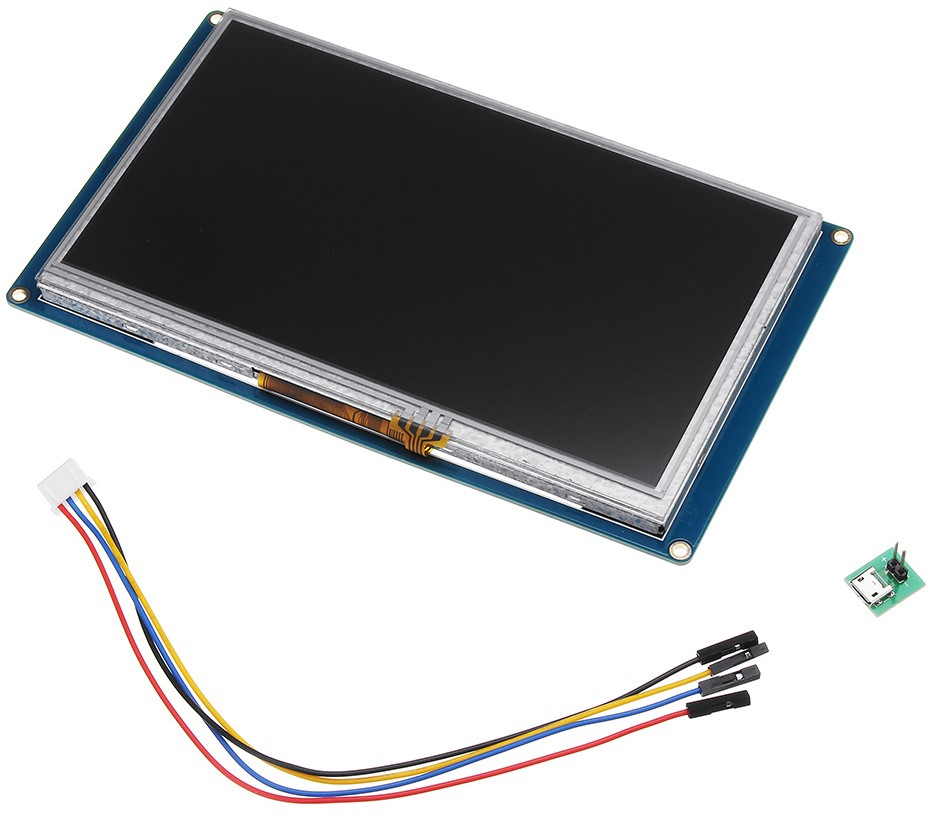
\includegraphics[width=0.7\textwidth]{graphics/Nextion_Display.jpg}
\caption{Ansichtsbild des verwendeten Display's. \cite{made-in-china_nextion_nodate}}
\label{fig:Nextion_Display}

\end{figure}

Um mit diesem Displaytyp arbeiten zu können, ist es wichtig, dass man sich einen Überblick über die Eigenschaften verschafft. Die wichtigsten Eigenschaften des Display's können in Tablle \ref{tab:Eigenschaften_Nextion_Display} eingesehen werden.

\begin{table}[h!]
\centering
\begin{tabularx}{0.6\textwidth}{|X|p{2.8cm}|}
\hline
\textbf{Speisespannung:} & 5V
\\
\hline
\textbf{Arbeitsstrom:} & 510mA
\\
\hline
\textbf{Sleep-Mode Strom:} & 15mA
\\
\hline
\textbf{Arbeitstemperatur:} & -20\textdegree bis 70\textdegree
\\
\hline
\textbf{Flash Speicher:} & 16MB
\\
\hline
\textbf{RAM Speicher:} & 3584BYTE
\\
\hline
\textbf{Farben:} & 65536 Farben
\\
\hline
\textbf{Auflösung:} & 800*480
\\
\hline
\textbf{Touch Typ:} & resistiv
\\
\hline
\textbf{Hintergrundbeleuchtung:} & LED
\\
\hline
\end{tabularx}
\caption{Eigenschaften des Nextion Display's \cite{patrick_nx8048t070_nodate}.}
\label{tab:Eigenschaften_Nextion_Display}
\end{table}

Die zwei grössten Vorteile dieses Displaytyps sind die Entwicklungsumgebung, sowie die grosse Community. Nextion bietet von sich aus einen GUI-Editor (Graphical User Interface Editor) an, welcher gratis zur Verfügung gestellt wird. Mit Hilfe dieses Tools können spielend leicht grafische Oberflächen geschaffen werden mit verschiedensten Komponenten wie Tasten, Textfelder, Bilder, Slider und viele mehr. Die Oberfläche des Editors kann in Abbildung \ref{fig:Nextion_Editor} begutachtet werden.

\begin{figure}[h!]
\centering
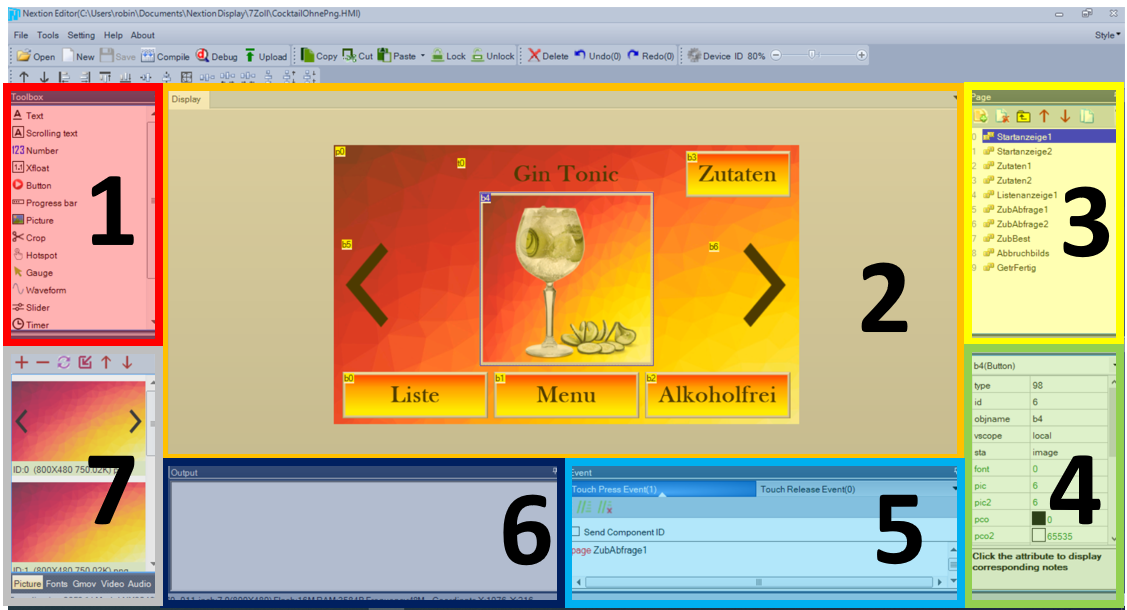
\includegraphics[width=\textwidth]{graphics/Nextion_Editor.png}
\caption{Entwicklungsumgebung von Nextion (Nextion Editor).}
\label{fig:Nextion_Editor}
\end{figure}

Die Software ist so einfach wie möglich gehalten. Im roten Feld 1 können Komponenten wie Slider, Textfelder, Tasten ect. per Klick in die erstellte Displayoberfläche im orangen Feld 2, im Ansichtsfenster eingefügt werden. In diesem Feld ist zu sehen, was schlussendlich auf dem Display ersichtlich ist. Es können natürlich mehrere Displayseiten erstellt werden. Diese können im gelben Feld 3 hinzugefügt, gelöscht oder umbenannt werden. Per Klick auf die gewünschte Seite wird diese im Ansichtsfenster 2 angezeigt und kann dann bearbeitet werden. Im grünen Feld 4 befinden sich die Eigenschaften der Elemente der erstellten Displayseite. Wird ein Element auf der Displayseite angeklickt, so erscheinen dort dessen Eigenschaften. Diese können dann beliebig angepasst werden. Dazu gehören zum Beispiel die Elementgrösse oder die Platzierungsposition. Im blauen Feld 5 kann den einzelnen Elementen ein Reaktionsbefehl gegeben werden. Dabei kann ausgewählt werden, ob das Element auf Drücken, Loslassen oder beides Reagieren soll. Ausserdem können dort Befehle eingegeben werden. Also zum Beispiel bei einem Taster: ``page 2``. Dies bedeutet so viel wie: ``Falls das Element gedrückt wird, dann zeige Displayseite 2 an``. Natürlich können so auch Befehle über die UART-Schnittstelle weiter gegeben und empfangen werden. Das violette Feld 6 bietet eine Outputübersicht an, welche zu Simulationszwecken verwendet wird. Im letzten grauen Feld 7 können Vorlagen abgespeichert werden. Dazu gehören Bilder, Textstyle Vorlagen, Audio- und Videodateien.